\documentclass[11pt,reqno]{amsart}

% packages


\usepackage[top=3cm,bottom=3cm,left=3cm,right=3cm]{geometry}
\usepackage{hyperref}

\usepackage{graphicx}
% THEOREM Environments ---------------------------------------------------

\newtheorem{theorem}{Theorem}[section]
 \newtheorem{corollary}[theorem]{Corollary}
 \newtheorem{lemma}[theorem]{Lemma}
 \newtheorem{proposition}[theorem]{Proposition}
 \newtheorem{conjecture}{Conjecture}
  \newtheorem{question}{\sc Question}

  \theoremstyle{definition}
 \newtheorem{definition}[theorem]{Definition}
 \newtheorem{example}[theorem]{Example}

 \theoremstyle{remark}
 \newtheorem{remark}[theorem]{Remark}


\numberwithin{equation}{section}

\newcommand{\C}{\mathbb{C}}
\renewcommand{\t}{{\bf t}}
\newcommand{\fulges}[1]{{\color{cyan} #1}}
%\renewcommand{\St}{\mathfrak{St}}
\usepackage{diagbox}


\title{Problems and Exercises}

\author{P. Breiding, T. Brysiewicz, S. Telen, S. Timme}


\begin{document}
\maketitle
\tableofcontents

\section{Coding exercises}

\begin{enumerate}
\item A conic is the zero set of a quadratic polynomial
$$
c(x,y) = a_1 x^2 + a_2 x y + a_3 y^2 + a_4 x + a_5 y + a_6
$$
with $a_i \in \mathbb{C}$.

\href{http://www.win.tue.nl/EWCG2005/Proceedings/38.pdf}{Emiris and Tzoumas} showed that there are 184 complex circles that are tangent to 3 general conics $C_1$, $C_2$ and $C_3$. This means, that there are 184 complex solutions $(a_1,a_2,r)$ such that there exists some $(x,y)\in\mathbb{C}^2$ with
\begin{align*}
&(x-a_1)^2 + (y-a_2)^2 = r\\
&(x,y)\in C_i \text{ for } \leq i\leq 3\\
&(x-a_1, y-a_2) \text{ spans the normal space of $C_i$ at $(x,y)$ for $1\leq i\leq 3$.}
\end{align*}

\begin{enumerate}
\item Define the polynomial system for 3 general conics and verify that this system has indeed 184 solutions. Use certification.

\item
Consider the three conics

\begin{align*}
&C_1 = \{y=-x^2+2x+5\},\\
&C_2 = \{y = 2x^2+5x-8\},\\
&C_3 = \{y = 8x^2-3x-2\}.
\end{align*}

How many circles are tangent to these 3 conics? How many of them are real?

\item Find a configuration of 3 conics with as many real solutions as possible. It is possible to find 184 real solutions?

\end{enumerate}

\item A real algebraic variety is the common zero set of polynomials $f_1, \ldots, f_m \in \mathbb{R}[x_1,\ldots,x_n]$ denoted by $X=V(f_1,\ldots,f_m)$. A bottleneck of $X$ is defined to be a pair of distinct points $x, y \in X$ such that $x-y$ is orthogonal to the tangent space $\mathrm{T}_x X$ and to $\mathrm{T}_y X$.

\href{https://arxiv.org/abs/1904.04502}{It was recently shown} that a generic plane curve of degree $d$ has $d^4-5d^2 +4d$ bottleneck pairs. This is called the {bottleneck degree} of the curve.


Consider the curve $X=V(f)$ defined by
$$f=(x^4 + y^4 - 1)(x^2 + y^2 - 2) + x^5y.$$
\begin{enumerate}
\item Write down definining equations for computing all bottlenecks.

\item What is the Bottleneck degree of $X$? How many real bottlenecks does it have?

\item What are the coordinates smallest bottleneck pair?

\item What effect do different start systems have on the number of paths necessary to track?
\end{enumerate}

\item Consider a general quartic surface $X\in\mathbb C^3$.  This is defined by a random polynomial $f\in \mathbb{C}[x,y,z]$ of degree 4. HC.jl provides  \href{https://www.juliahomotopycontinuation.org/HomotopyContinuation.jl/stable/model_kit/}{functions to sample random polynomials}. We want to count the number of planes in three-space which are tangent to $f=0$ in at least 3 points.
\begin{enumerate}
\item Set up polynomial systems to compute all tritangent planes of a general quartic surface. (\textit{Hint: you should obtain a polynomial system in 11 variables}).
\item Use monodromy to solve the system from (a).
\end{enumerate}

\item Extend the \href{https://www.juliahomotopycontinuation.org/examples/computer-vision/}{triangulation} example from two to three (or more) cameras.

\item Verify that the configurations of 5 conics at \href{https://www.juliahomotopycontinuation.org/examples/3264/}{this link} has 3264 real conics, which are simultaneously tangent to all 5 of them. Use certification methods to obtain a proof!

\item A quintic threefold is the zero set $X=\{(x,y,z,w)\in\mathbb C^4\mid f(x,y,z,w)=0\}$ of a polynomial $f\in\mathbb C[x,y,z,w]$ of degree $5$. Let $X$ be a quintic threefold defined by a randomly chosen polynomial $f$. Then, $X$ contains finitely many lines. Compute them. How many are there?

\item Consider three Gaussian random variables $X_1,X_2,X_3$ with means $\mu_1,\mu_2,\mu_3$ and variances $\sigma_1^2,\sigma_2^2,\sigma_3^2$. The density of $X_i$ is
$$\phi_i(x) = \frac{1}{\sqrt{2\pi}} e^{-\frac{(x-\mu_i)^2}{2\sigma_i^2}}.$$
A mixture of the three random variables is a random variable with density
$$\psi(x) = a_1 \phi_1(x) + a_2 \phi_2(x) + a_3 \phi_3(x), \quad\text{   for } \quad  a_1+a_2+a_3 =1.$$
The \href{https://en.wikipedia.org/wiki/Method_of_moments_(statistics)}{method of moments} recovers $\psi$ from the moments
  $$m_k = \int x^k \psi(x) \mathrm{d}x.$$
Since we have 9 unknowns plus one equation $a_1+a_2+a_3=1$, we expect to need at least 8 moments to recover $\psi$. Set up a system $F$ with variables $\mu_1,\mu_2,\mu_3$, $\sigma_1^2,\sigma_2^2,\sigma_3^2$ and $a_1,a_2,a_3$ that computes the first 8 moments of $\psi$. Then, randomly sample values for the 9 variables, evaluate $F$ at those values. This gives a vector $m\in \mathbb C^8$. Solve the system $F-m=0$ (see \href{https://www.juliahomotopycontinuation.org/examples/method-of-moments/}{here}, if you need help).

\item Describe the solution set to the system
\begin{align*}
(4s_4^2-2s_4s_6+4s_4s_7+6s_4s_8-2s_4-2s_6s_8+s_6+4s_7s_8+2s_8^2-s_8)y+\\
(-4s_2s_4-4s_2s_8+s_2-4s_4^2-4s_4s_6-8s_4s_8+3s_4-4s_6s_8+2s_6+2s_7- \\
4s_8^2+4s_8-1)z = 0.\\
(2s_6+4s_7+2s_8-1)z^2+(8s_2s_4^2+16s_2s_4s_8-4s_2s_4-s_2s_6-2s_2s_7+ \\
8s_2s_8^2-5s_2s_8+s_2+8s_4^3+16s_4^2s_7+16s_4^2s_8-8s_4^2+3s_4s_6+ \\
32s_4s_7s_8-2s_4s_7+8s_4s_8^2-9s_4s_8+s_4-s_6^2-2s_6s_7+2s_6s_8+\\
16s_7s_8^2-2s_7s_8-s_8^2) = 0.
\end{align*}
in the variables $s_2,s_4,s_6,s_7,s_8, y,z$ restricted to the locally closed set
$$\mathcal{C} = {V}_1-({V}_2\cap{V}_3)\cup({V}_4\cap{V}_5),$$
where ${V}_1$ is the solution set to
\begin{align*}
s_2^2+2s_2s_4+s_2s_6+2s_2s_7+s_2s_8-s_2+s_4^2+s_4s_6+2s_4s_7+s_4s_8-\\
s_4+2s_6s_7+2s_7s_8 = 0,
\end{align*}
and
\begin{align*}
{V}_2  &= \{2s_6+4s_7+2s_8-1 = 0\},\\
{V}_3  &= \{s_2+s_4-2s_7 = 0 = 0\},\\
{V}_4  &= \{4s_4^2-2s_4s_6+4s_4s_7+6s_4s_8-2s_4-2s_6s_8+s_6+4s_7s_8+2s_8^2-s_8  = 0\},\\
{V}_5  &= \{s_2-s_4+s_6-s_8 = 0\},
\end{align*}
(submitted by Ernesto \'{A}lvarez Gonz\'{a}lez.)
\end{enumerate}

\section{Witness Sets}
\begin{enumerate}
\item Prove the trace test for plane curves. i.e. prove
\begin{itemize}
\item if $C=\mathcal{V}(f(x,y))$ is an irreducible curve, and $L_t$ a generic parallel family of lines, then the sum of the points $C \cap L_t$ moves linearly in $t$. \\ (Hint: assume $L_t$ are the lines $\mathcal{V}(x-t)$)

\item if $S_t$ is a proper subset of $C \cap L_t$, then the sum of the points in $S_t$ moves nonlinearly as $t$ moves. \\ (Hint: the monodromy of the points $C \cap L_t$, as $t$ moves, is the full symmetric group)
\end{itemize}

\item How many maximal dimensional irreducible components does
$$\text{HSO}(4) = \{M \in \text{Mat}_{\mathbb{C}}(4,4) \mid MM^T= \textrm{id}, \det(M) = 1, M_{i,i}=0 \text{ for all }i\}$$
have? What are their degrees? How do they intersect?


\item Given a surface $X \subset \mathbb{R}^3$, the {\textit{flecnodal surface}} $\mathcal{F}(X)$ is the union of all lines $L$ with contact order $4$ at a point of $X$. It is one of five {\textit{event surfaces}} described in \href{https://arxiv.org/pdf/1707.01877.pdf}{ ``Changing views on curves and surfaces"} by Kohn, Sturmfels, and Trager.
\begin{itemize}
\item A quintic polynomial $$f=c_5+c_4t+\cdots+c_1t^4+c_0t^5$$ has a root of multiplicity four whenever the coefficients satisfy
\begin{align*}
20c_0c_4-8c_1c_3+3c_2^2&=0 \\
50c_0c_5-6c_1c_4+c_2c_3&=0 \\
20c_1c_5-8c_2c_4+3c_3^2&=0.
\end{align*}
Compute a witness set for the above equations. For each witness point, solve the corresponding polynomial and observe that one root comes with multiplicity four.
\item Consider the quintic surface $$f = x_1^5+x_2^5+x_3^5+1+(x_1+x_2+x_3+1)^5+x_1x_2x_3(x_1+x_2+x_3+1)$$
in $\mathbb{R}^3$. Find a suitable parametrization for lines in $\mathbb R^3$., Compute a witness set for the Flecnodal surface of $X=\mathcal{V}(f)$. What is its degree?
\item We can pass from $\mathbb R^3$ to projective space $\mathbb P^3$. Here, lines can be parametrized using Pl\"ucker coordinates $\{q_{1,2},q_{1,3},q_{1,4},q_{2,3},q_{2,4},q_{3,4}\}$:
$$z(t) = (q_{1,2}:tq_{1,2}:tq_{1,3}-q_{2,3}:tq_{1,4}-q_{2,4})$$
Homogenize $f(x_1,x_2,x_3)$ to $f_\mathrm{hom}(x_0,x_1,x_2,x_3)$ and compute a witness set for the Flecnodal surface of $X=\mathcal{V}(f_\mathrm{hom})$ in the coordinates $q$ (remember to include the Pl\"ucker relation $q_{1,2}q_{3,4}-q_{1,3}q_{2,4}+q_{1,4}q_{2,3}=0$.) What is its degree?
\end{itemize}




\end{enumerate}


\section{Total degree and polyhedral homotopies}

\begin{enumerate}
\item (Conics in the plane). Consider the total degree family $\mathcal{F}(2,2)$, i.e.~$n = 2$ and $(d_1, d_2) = (2,2)$:

$$ \mathcal{F}(2,2) = \begin{pmatrix}
f_1 \\ f_2
\end{pmatrix}  = \begin{pmatrix}
a_{00} + a_{10} x + a_{01} y + a_{20}x^2 + a_{11}xy + a_{02} y^2 \\
b_{00} + b_{10} x + b_{01} y + b_{20}x^2 + b_{11}xy + b_{02} y^2 \\
\end{pmatrix}. $$
\begin{figure}[!htpb]
\centering
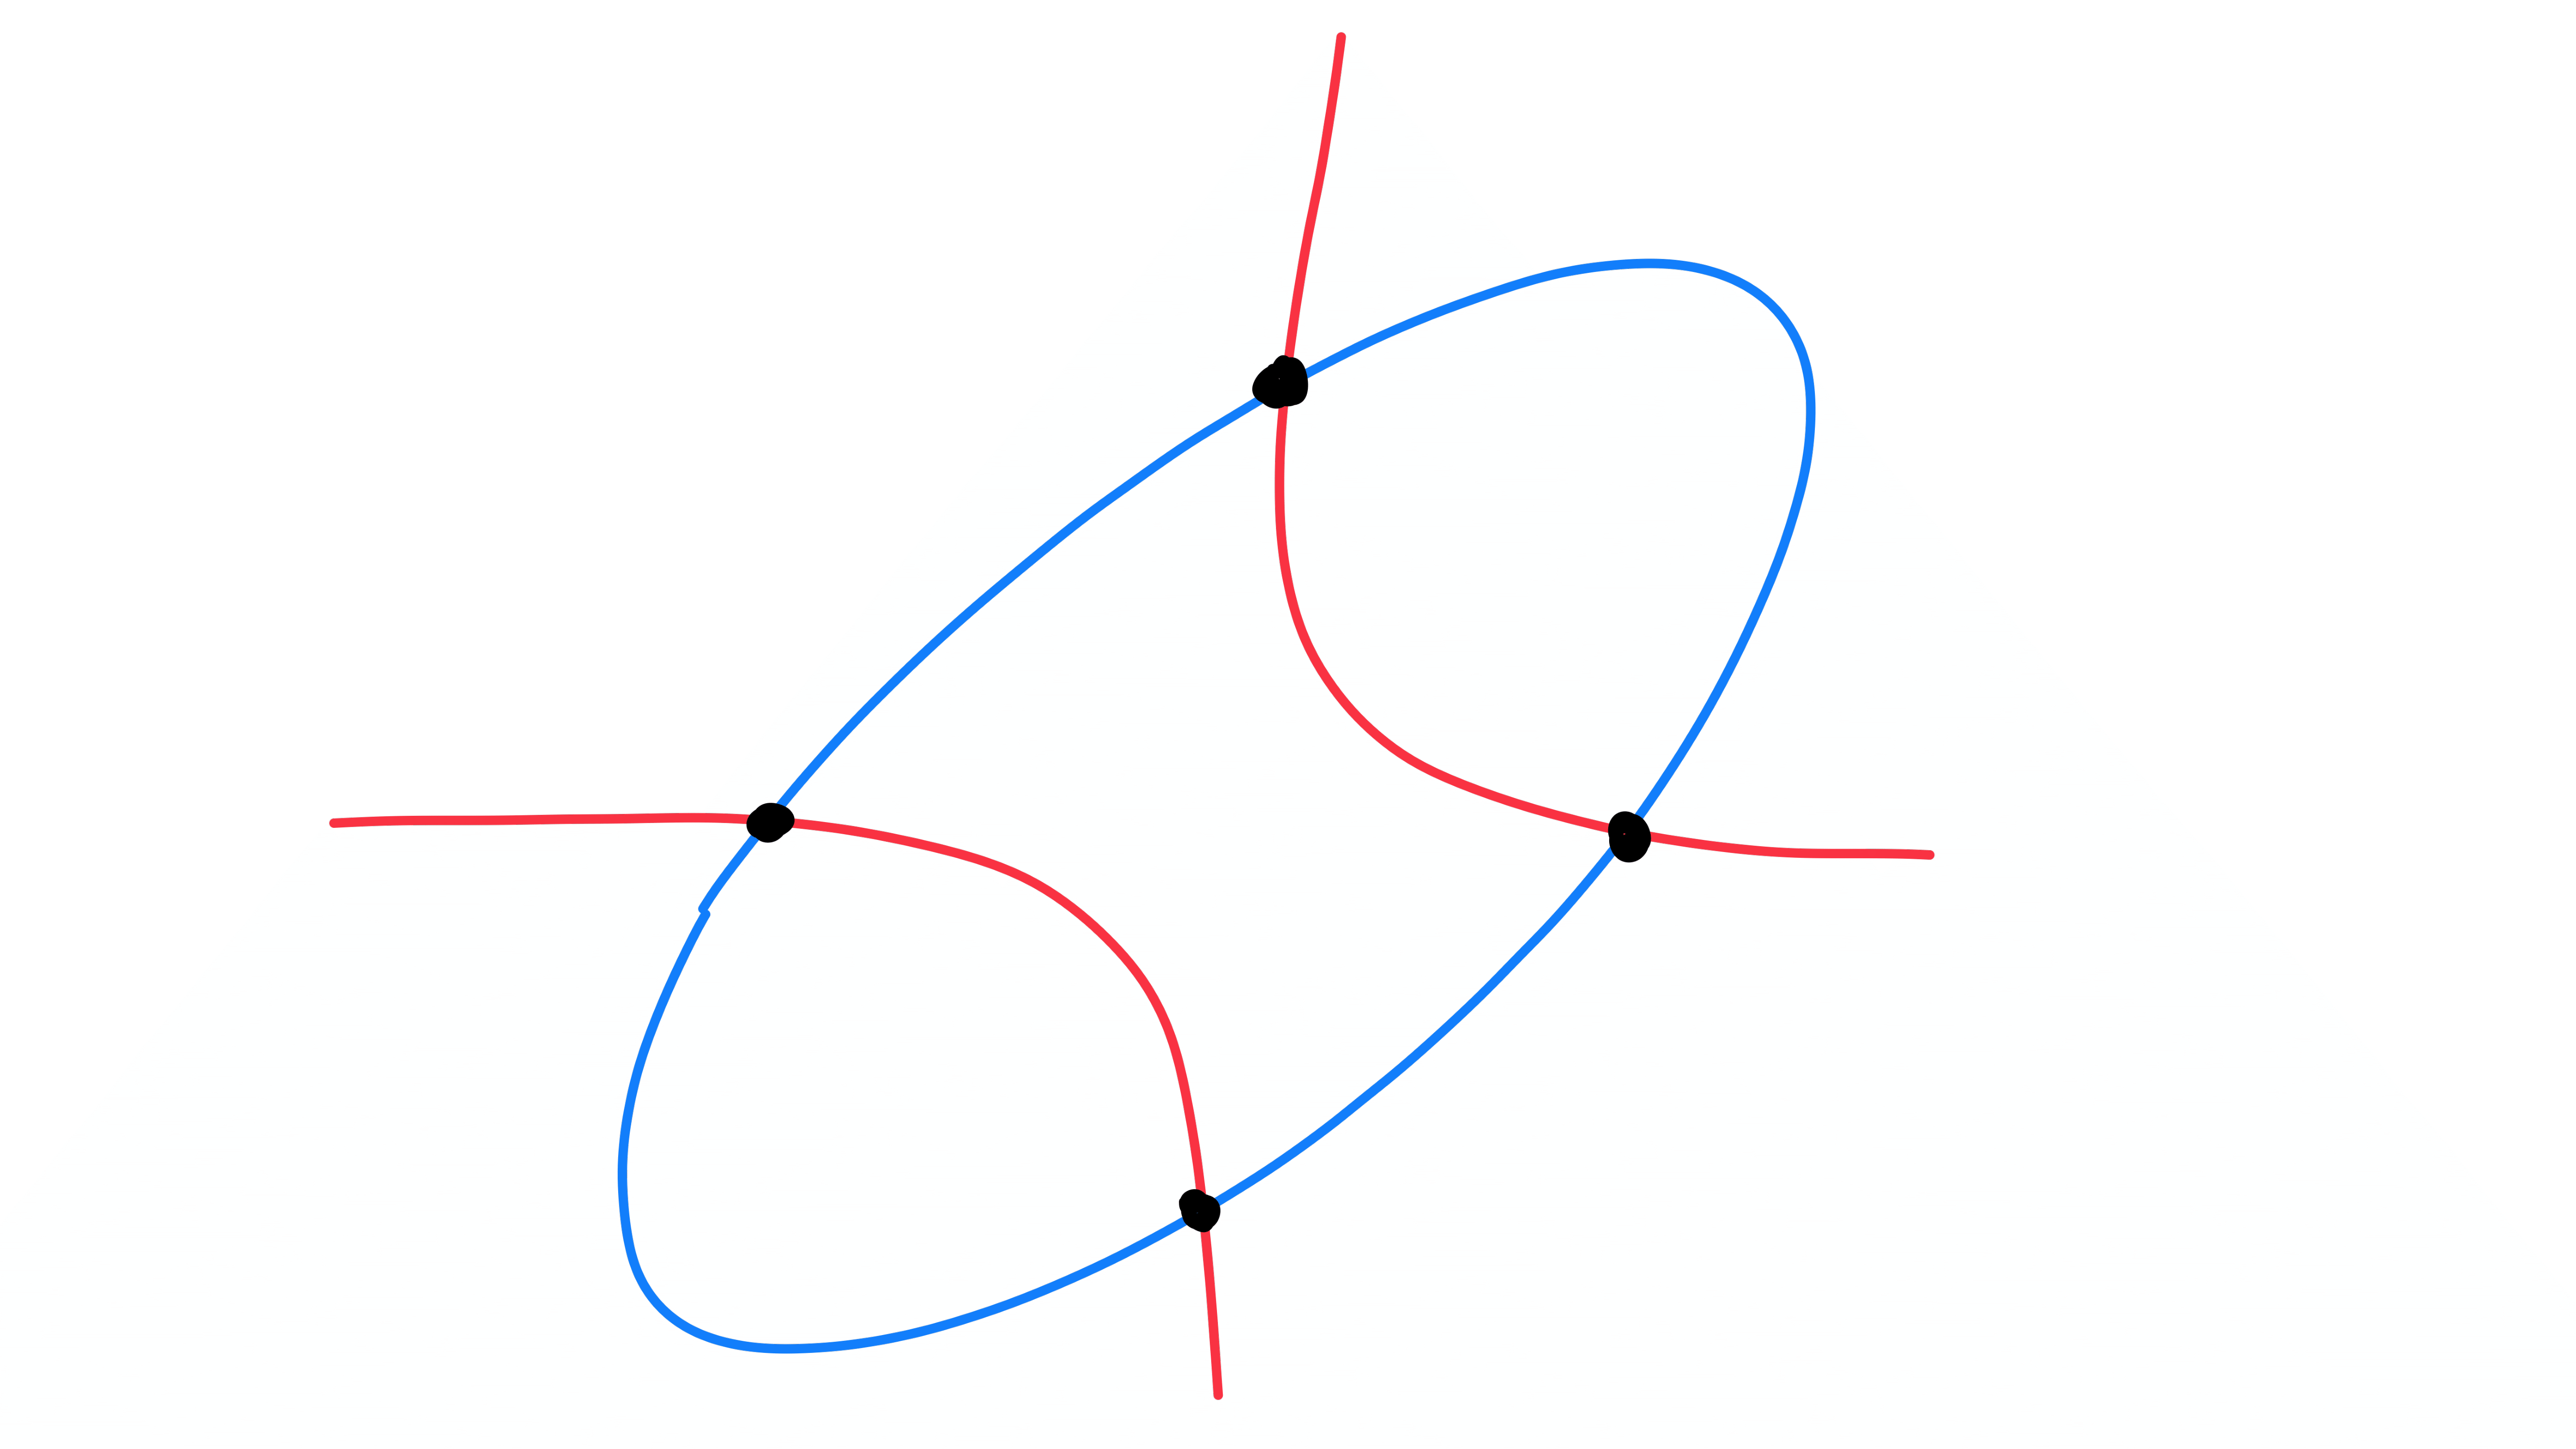
\includegraphics[scale=0.04]{Pictures_SANNA-4-1.png}
\caption{Two \emph{generic} conics in the plane.}
\end{figure}
What is $\mathcal{N}_{\text{Béz}}$ in this example? Verify this by solving a random member of this family using \texttt{HomotopyContinuation.jl}.

There are strictly less than $\mathcal{N}_{\text{Béz}}$  solutions in the following two scenarios.

\begin{itemize}
\item Two or more solutions \emph{coincide}. This happens if there are solutions to the overdetermined system
$$ f_1 = f_2 = \det \begin{pmatrix} f_{1x} & f_{1y} \\ f_{2x} & f_{2y} \end{pmatrix} = 0 \quad \text{has a solution}.$$
Here $f_{ix} = \partial f_i / \partial x$ and likewise for $f_{iy}$. Prove (possibly using a computer algebra system) that this is equivalent to the vanishing of a nonzero polynomial in the coefficients of $f_1, f_2$. This polynomial is called the \emph{discriminant}.
\item There are solutions \emph{at infinity}. To make this precise, we homogenize the equations:
$$\begin{pmatrix}
a_{00} z^2+ a_{10} x z+ a_{01} yz + a_{20}x^2 + a_{11}xy + a_{02} y^2 \\
b_{00} z^2 + b_{10} x z + b_{01} yz + b_{20}x^2 + b_{11}xy + b_{02} y^2 \\
\end{pmatrix},$$
and consider solutions with $z = 0$. Geometrically, we replace our conics by their closures in $\mathbb{P}^2$. Show that there are solutions `at infinity' if and only if
$$ \det A_\infty = \det \begin{pmatrix} a_{20} & a_{11} & a_{02} & \\ & a_{20} & a_{11} & a_{02} \\ b_{20} & b_{11} & b_{02} & \\ & b_{20} & b_{11} & b_{02} \end{pmatrix} = 0.$$
\end{itemize}
What about the case where $f_1 = f_2 = 0$ has infinitely many solutions? \\

Construct two members of $\mathcal{F}(2,2)$ with 3 solutions, one with a solution at infinity, and one with a solution of multiplicity 2. Verify using \texttt{HomotopyContinuation.jl}.

\item (Systems supported on the square).
Consider the subfamily
$$ \mathcal{F}_Q = \begin{pmatrix}
f_1 = a_{00} + a_{10}x + a_{10}y + a_{11}xy \\
f_2 = b_{00} + b_{10}x + b_{10}y + b_{11}xy \\
\end{pmatrix} \subset \mathcal{F}(2,2).$$
Use the previous exercise to show that $\mathcal{N}(Q) < \mathcal{N}_{\textup{B\'ez}}$. Verify the formula $\text{MV}(P_1,P_2) = \text{Vol}_2(P_1 + P_2) - \text{Vol}_2(P_1) - \text{Vol}_2(P_2)$ for $P_1 = P_2 = [0,1]^2 \subset \mathbb{R}^2$. More generally, compute $\text{MV}(P_1, \ldots, P_n)$ with $P_i = [0,1]^n \subset \mathbb{R}^n$ for all $i$. This corresponds to a sparse family $\mathcal{F}_Q \subset \mathcal{F}(n,\ldots, n)$. Compare $\mathcal{N}(Q)$ for these systems with their B\'ezout number. For some $n$, solve a generic member of $\mathcal{F}_Q$ using a total degree and a polyhedral start system in \texttt{HomotopyContinuation.jl}.

\item (Asymptotic BKK and B\'ezout numbers).
This is an example taken from \href{https://www.jstor.org/stable/2153370?seq=1#metadata_info_tab_contents}{ ``A polyhedral method for solving sparse polynomial systems"} by Birkett Huber and Bernd Sturmfels. Consider the family

$$\begin{pmatrix}
a_1 +  a_2 x + a_3 x^ky^k \\
b_1 + b_2 y + b_3 x^ky^k
\end{pmatrix} \subset \mathcal{F}(2k,2k).$$
Show that $\lim_{k \rightarrow \infty} ( \mathcal{N}_{\text{BKK}} / \mathcal{N}_{\text{Béz}} ) = 0$. Compare the computation time for the function \texttt{solve} in \texttt{HomotopyContinuation.jl} using the default option (\texttt{start\_system = :polyhedral}) and the option \texttt{start\_system = :total\_degree} for random coefficients $a, b$ and increasing values of $k$.

 \item (Toric varieties and the BKK theorem).
Let $\mathcal{A} = \{ \alpha_1, \ldots, \alpha_r \} \subset \mathbb{N}^n$ be a set of exponents such that $P = \text{Conv}(\mathcal{A})$ has dimension $n$. The \emph{projective toric variety} $X_\mathcal{A}$ associated to $\mathcal{A}$ is the Zariski closure of the image of the monomial map
$$ (x_1, \ldots, x_n) \mapsto (x^{\alpha_1} : \cdots : x^{\alpha_r}) \in \mathbb{P}^{r-1}.$$
Use the BKK theorem to relate the degree of $X_\mathcal{A}$ to the volume of $P$. The statement you obtain is known as \emph{Kushnirenko's theorem}, which can be seen as a specialized version of the BKK theorem for \emph{unmixed systems of equations}, for which $\mathcal{A}_i = \mathcal{A}, i = 1, \ldots, n$.

\item (Puiseux series solutions).
Consider the polynomial $f = tx^3 + 2x^2 + t \in K[x]$, where $K$ is the field of Puiseux series with complex coefficients in the variable $t$. Compute the leading term of all solutions $x \in K$ to $f = 0$. That is, compute all possible $X \in \mathbb{C} \setminus \{0\}$ and $e \in \mathbb{Q}$ such that there is a solution $x(t) = X t^e + \text{higher order terms}$ satisfying $f(x(t),t) = 0$.

\textit{Hint: substitute $x(t) = X t^e + \text{higher order terms}$ in $f(x(t),t)$ and look for all exponents $e$ for which at least two terms of $f(x(t),t)$ are of lowest order in $t$. Obtain $X$ from the condition that these lowest order terms cancel. }

Can you give a graphical interpretation of the numbers $e$ in terms of the Newton polygon of $f$?

\textit{Hint: draw the Newton polygon of $f$ as a polynomial in $x,t$. }


\item (Solving binomial systems is easy).
Consider the system of equations over the field $K$ of complex Puiseux series in $t$:
$$
F = \begin{pmatrix} 1 + 2 x^2 y + 3 xy^2  \\
5 + 2 tx  + 4 ty + 6 txy \end{pmatrix} = 0.
$$
How many solutions $(x(t),y(t))$ do you expect? Check that there exists a solution of the form $x(t) = X t^{-1} + \text{ higher order terms}$ and $y(t) = Y t^2 + \text{ higher order terms}$, where $(X,Y)$ is the solution of
$$ 1 + 2 X^2Y = 5 + 2X = 0 .$$
Find $e_1, e_2 \in \mathbb{Q}$ such that $x(t) = X t^{e_1} +  \text{ higher order terms}$ and $y(t) = Y t^{e_2} + \text{ higher order terms}$ gives a solution for each $(X,Y) \in (\mathbb{C} \setminus \{0\})^2$ satisfying
$$ 2 X^2 Y + 3 XY^2 = 5 + 6 XY = 0.$$
To solve this \emph{system of binomial equations}, we write it in the form
\begin{equation} \label{eq:binomsys}
XY^{-1} = -3/2, \quad XY = -5/6.
\end{equation}
We collect the exponent vectors in the columns of a matrix $A = \begin{pmatrix}
1 & 1 \\ -1 & 1
\end{pmatrix}$. There exist matrices $P, Q \in \mathbb{Z}^{2 \times 2}$ with an inverse defined over $Z$ (i.e.~$P$ and $Q$ are \emph{unimodular}) which diagonalize $A$:
\begin{equation} \label{eq:snf}
P A Q = \begin{pmatrix}
s_1 & \\
& s_2
\end{pmatrix}.
\end{equation}
This diagonal matrix is called the \emph{Smith normal form} of $A$. Denote $p_{ij}, q_{ij}$ for the entries of $P$ and $Q$ respectively. Show that the map $ (\mathbb{C} \setminus \{0\})^2 \rightarrow (\mathbb{C} \setminus \{0\})^2 $ given by
$$ (U,V) \mapsto (U^{p_{11}} V^{p_{21}}, U^{p_{12}} V^{p_{22}})$$
is invertible. Use this change of coordinates on $(\mathbb{C} \setminus \{0\})^2$ and the identity \eqref{eq:snf} to reduce \eqref{eq:binomsys} to an equivalent system of equations
$$ U^{s_1} = c_1, \qquad V^{s_2} = c_2.$$
Deduce that the number of solutions of \eqref{eq:binomsys} is $\det A$. Can you write down an algorithm for solving a system of binomial equations in the form \eqref{eq:binomsys} with exponent matrix $A \in \mathbb{Z}^{n \times n}$?

We have now found the leading term of 3 solutions to $F = 0$. Can you find the missing solution(s) as well?
\end{enumerate}
\section{Monodromy}
Let $F_c(x)$ be a zero-dimensional parametrized polynomial system with variables $x_1,\ldots,x_n$ and parameters $c_1,\ldots,c_k$. Let $Z \xrightarrow{\pi} \C^k$ be the branched cover where $Z=\{(x,p) | F_p(x)=0\}$ and $\pi:Z \to \C^k$ is the projection onto the parameters. Let $d$ be the degree of this branched cover.
Let $U$ be the set of regular values of $\pi$ and $G_\pi$ the monodromy group based at some point $p \in U$.

\begin{enumerate}
\item Show $G_\pi$ is a group and it doesn't depend on the choice of $p \in U$ where you base monodromy loops.

\item Show $G_\pi$ is transitive if and only if $Z$ has a unique irreducible component of maximal dimension. Explain why $G_\pi$ being transitive is exactly the condition which allows \texttt{monodromy solve} to find all solutions to $\pi^{-1}(p)$.


\item Suppose $F_c(x)$ is defined over the real numbers.
\begin{itemize}
\item  Is it possible for a real path in $U$ to produce a nontrivial monodromy permutation?
\item Give an example.
\item  What does this tell you about the branch locus?
\end{itemize}

\item Consider the sparse polynomial system

$$\begin{pmatrix}
a_0+a_1x^2+a_2y^2+a_3x^2y^2 \\
b_0x+b_1x^3+b_2xy^2\\
\end{pmatrix},$$
\begin{itemize}
\item For $1000$ parameter values, solve this system and count how many real solutions you find.
\item Compute the Galois group over the parameters $\{a_0,a_1,a_3,a_4,b_0,b_1,b_2\}$.
\item What is the structure of this system that explains what you've observed?
\end{itemize}
\end{enumerate}




\end{document}
